\documentclass{slide}

% \usepackage{pgfpages}
% \setbeameroption{show notes on second screen}

\title{Architectural Skills}
\subtitle{CSSE6400}
\author{Richard Thomas}
\date{\week{13}}

\begin{document}

\maketitle

\point[Quote]{Architecture is the stuff you can't Google.\\
 ~~~~~ -- Mark Richards \cite{richards2020fundamentals}}

\point[Quote]{There are no right or wrong answers in architecture---only trade-offs.\\
 ~~~~~ -- Neal Ford \cite{richards2020fundamentals}}

\point[Architectural Design]
{Architects use knowledge and experience to analyse trade-offs to design architectures appropriate to the system context.}

\begin{frame}{Developers -- Technical Depth \cite{richards2020fundamentals}}
    \centering
    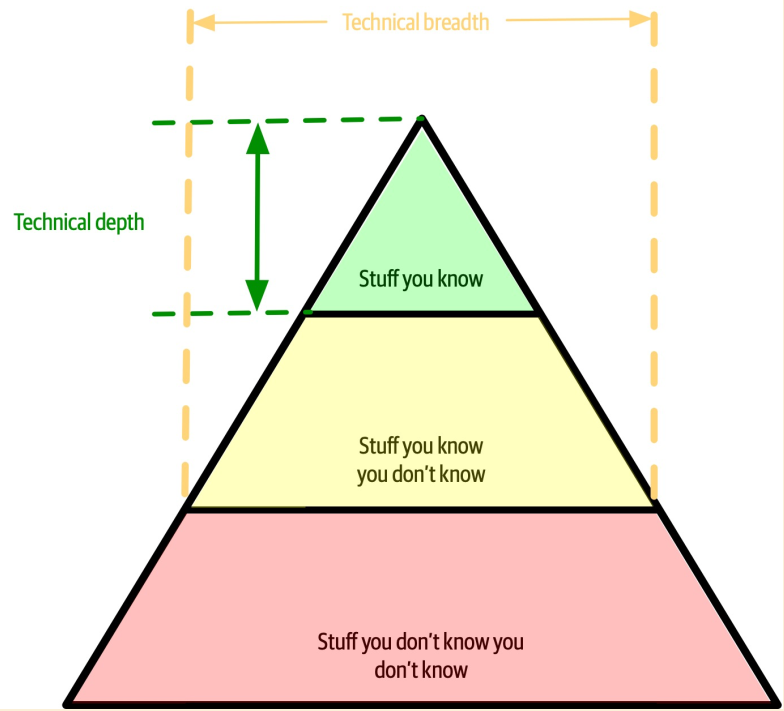
\includegraphics[trim=1 1 1 1,clip,height=0.92\textheight]{images/depth-breadth-pyramid-1.png}
\end{frame}

\begin{frame}{Architects -- Technical Breadth \cite{richards2020fundamentals}}
    \centering
    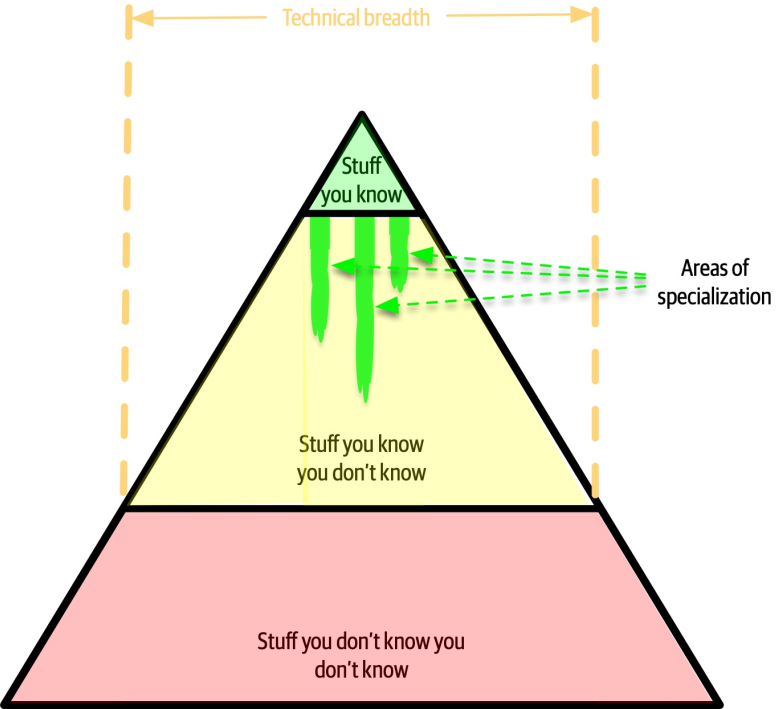
\includegraphics[trim=1 1 1 1,clip,height=0.92\textheight]{images/depth-breadth-pyramid-2.png}
\end{frame}
\note[itemize]{
    \item Architects need greater technical breadth than depth.
    \item Breadth allows better consideration of trade-offs.
    \item Avoid trying to become an expert across many areas -- you'll fail.
    \item Don't stop learning -- increase your breadth -- don't let your knowledge become stale.
}

\definition{Conway's Law}
{Organisations design systems whose structure is inevitably a copy of the organisation's communication structure \cite{conways-law} \cite{maccormack2012}.}
\note[itemize]{
    \item First citation is original article.
    \item Second citation is one of several about MIT and Harvard research into the phenomenon, calling it the ``mirroring hypothesis''.
    \item Elaborate on this point and Coplien's research into organisational sociology.
}

\point[Conway's Law Consequences]{
\begin{itemize}
    \item Business Process Management
    \vspace{2mm}
    \item Microservices to reflect organisation structure
    \vspace{2mm}
   \item Teams formed around services
\end{itemize}
}
\note[itemize]{
    \item BPM: Redesign organisation structure to reflect system you want.
    \item Microservices: Design system to reflect your organisation.
    \item Elaborate on benefits of both approaches.
    \item Comment on benefits of small focussed teams.
}

\point[Conway's Law Consequences]{Team insularity -- more loyal to team than organisation.}
\note[itemize]{
    \item Amazon example from week 11, negotiation difficulties with other teams.
    \item Need to ensure inter-team cooperation.
    \item Possibly move people between teams.
    \item Cloud platforms, and microservices, also support this and with larger teams.
    \item Intra-team communication becomes more difficult with large teams.
}

\begin{frame}{Conway's Law Issues}
\vspace{1pt}
{\huge
\begin{itemize}
    \item Cross-cutting concerns
    \begin{itemize}
        \LARGE\item e.g. Security
    \end{itemize}
    \vspace{2mm}
    \item Organisation structure should align with market structure
    \vspace{2mm}
    \item Physical location of teams
\end{itemize}
}
\end{frame}
\note[itemize]{
    \item Cross-cutting concerns span services, and consequently teams.
    \item Can't have a ``security'' service. It has to be part of every service.
    \item Teams solely based around Conway's law and services may not deliver some cross-cutting concerns.
    \item Cooperation, documentation and audits may be necessary.
    \item Market structure may complement team structure to place teams closer to their end users.
    \item Global development and outsourcing mean different teams are likely to be in different locations.
    \item Requires additional overhead and documentation for cooperation between teams.
}

\point[Evidenced-Based Software Engineering]{Don't follow fads, seek evidence for good practice.}
\note{Elaborate on finding reliable sources of information and confirming facts yourself.}

\point[Let's hear from an expert]{\centering \youtubevideo{images/se-hits-thumb}{https://youtu.be/HrVtA-ue-x0}}

\references{books,articles}

\end{document}